\chapter{Control, Simulation, and Visualization Software}
\label{ch:software}

\section{Visualizer}

The Eelume Visualizer refers to software developed as part of this thesis to 
visualize the pose of the Eelume robot in real time during experimental 
operations. The necessity for such a tool became apparent during initial 
testing on the Eelume robot. The default software suite used for Eelume 
provides a map view of the robot's position and displays Euler angles, position,
and joint angles as numerical values on a screen. This setup makes it 
difficult to gain a quick and intuitive understanding of the robot's current 
configuration, particularly in observing how it evolves over time. The Eelume 
Visualizer addresses this issue by presenting a real-time computer-generated 
rendering of the robot.

% features
The visualizer offers a wide range of features. The rendering of the Eelume 
robot is based on 3D object files supplied by Eelume AS, which enhances the 
realism of the visualization. Joints can be configured to arbitrary angles, 
and their motion is accurately represented through the bending of the 
connected links. The visualizer includes a grid in the north-east plane and 
displays an \gls{ned} axis at the coordinate origin, providing spatial context 
and aiding in visualizing depth and orientation. Additionally, it supports 
rendering spheres of arbitrary color and position, which has been extensively 
used to depict desired task values. This allows users to intuitively assess 
how effectively a controller is executing a task without needing to analyze 
numerical data.

The visualizer supports switching between different fields of view and 
projection methods, including both perspective and orthographic projections. 
When appropriately positioned, the camera also enables an isometric view. 
These capabilities make the visualizer well-suited for professional 
presentation of specific Eelume configurations. In fact, all computer-
generated imagery of the Eelume robot presented in this thesis was created 
using the visualizer. It includes built-in screenshot functionality, allowing 
for the export of images with a transparent background (\(0\) alpha value). An 
optional shadow projection feature enhances spatial perception by casting a 
shadow onto the virtual ground plane.

% how it was made
The visualizer is implemented in pure C++ using OpenGL in conjunction with the 
GLEW and GLFW libraries. All shaders, which manage scene lighting, are written 
in the OpenGL shading language \textit{GLSL} and were developed as part of 
this thesis. This includes custom shading for the joints, which required 
specialized mathematical treatment to bend accurately. These joint shaders 
were implemented using the matrix exponential of \(\se\) elements, as 
described mathematically in \autoref{ch:appendix:math}.

% how it works (udp)
The robot's position, along with the color and position of the spheres, is 
controlled externally through messages sent via \gls{udp}. This allows for 
straightforward integration and control from virtually any programming language
. A lightweight C++ header file was created to expose functions for setting 
the robot's pose and rendering spheres.

An example of the visualizer in use during an experiment is shown in
\autoref{fig:eelume:visualizer}. The background grid lines and the central
axis system illustrate the origin of the \gls{ned} frame.
\begin{figure}[h!]
    \centering
    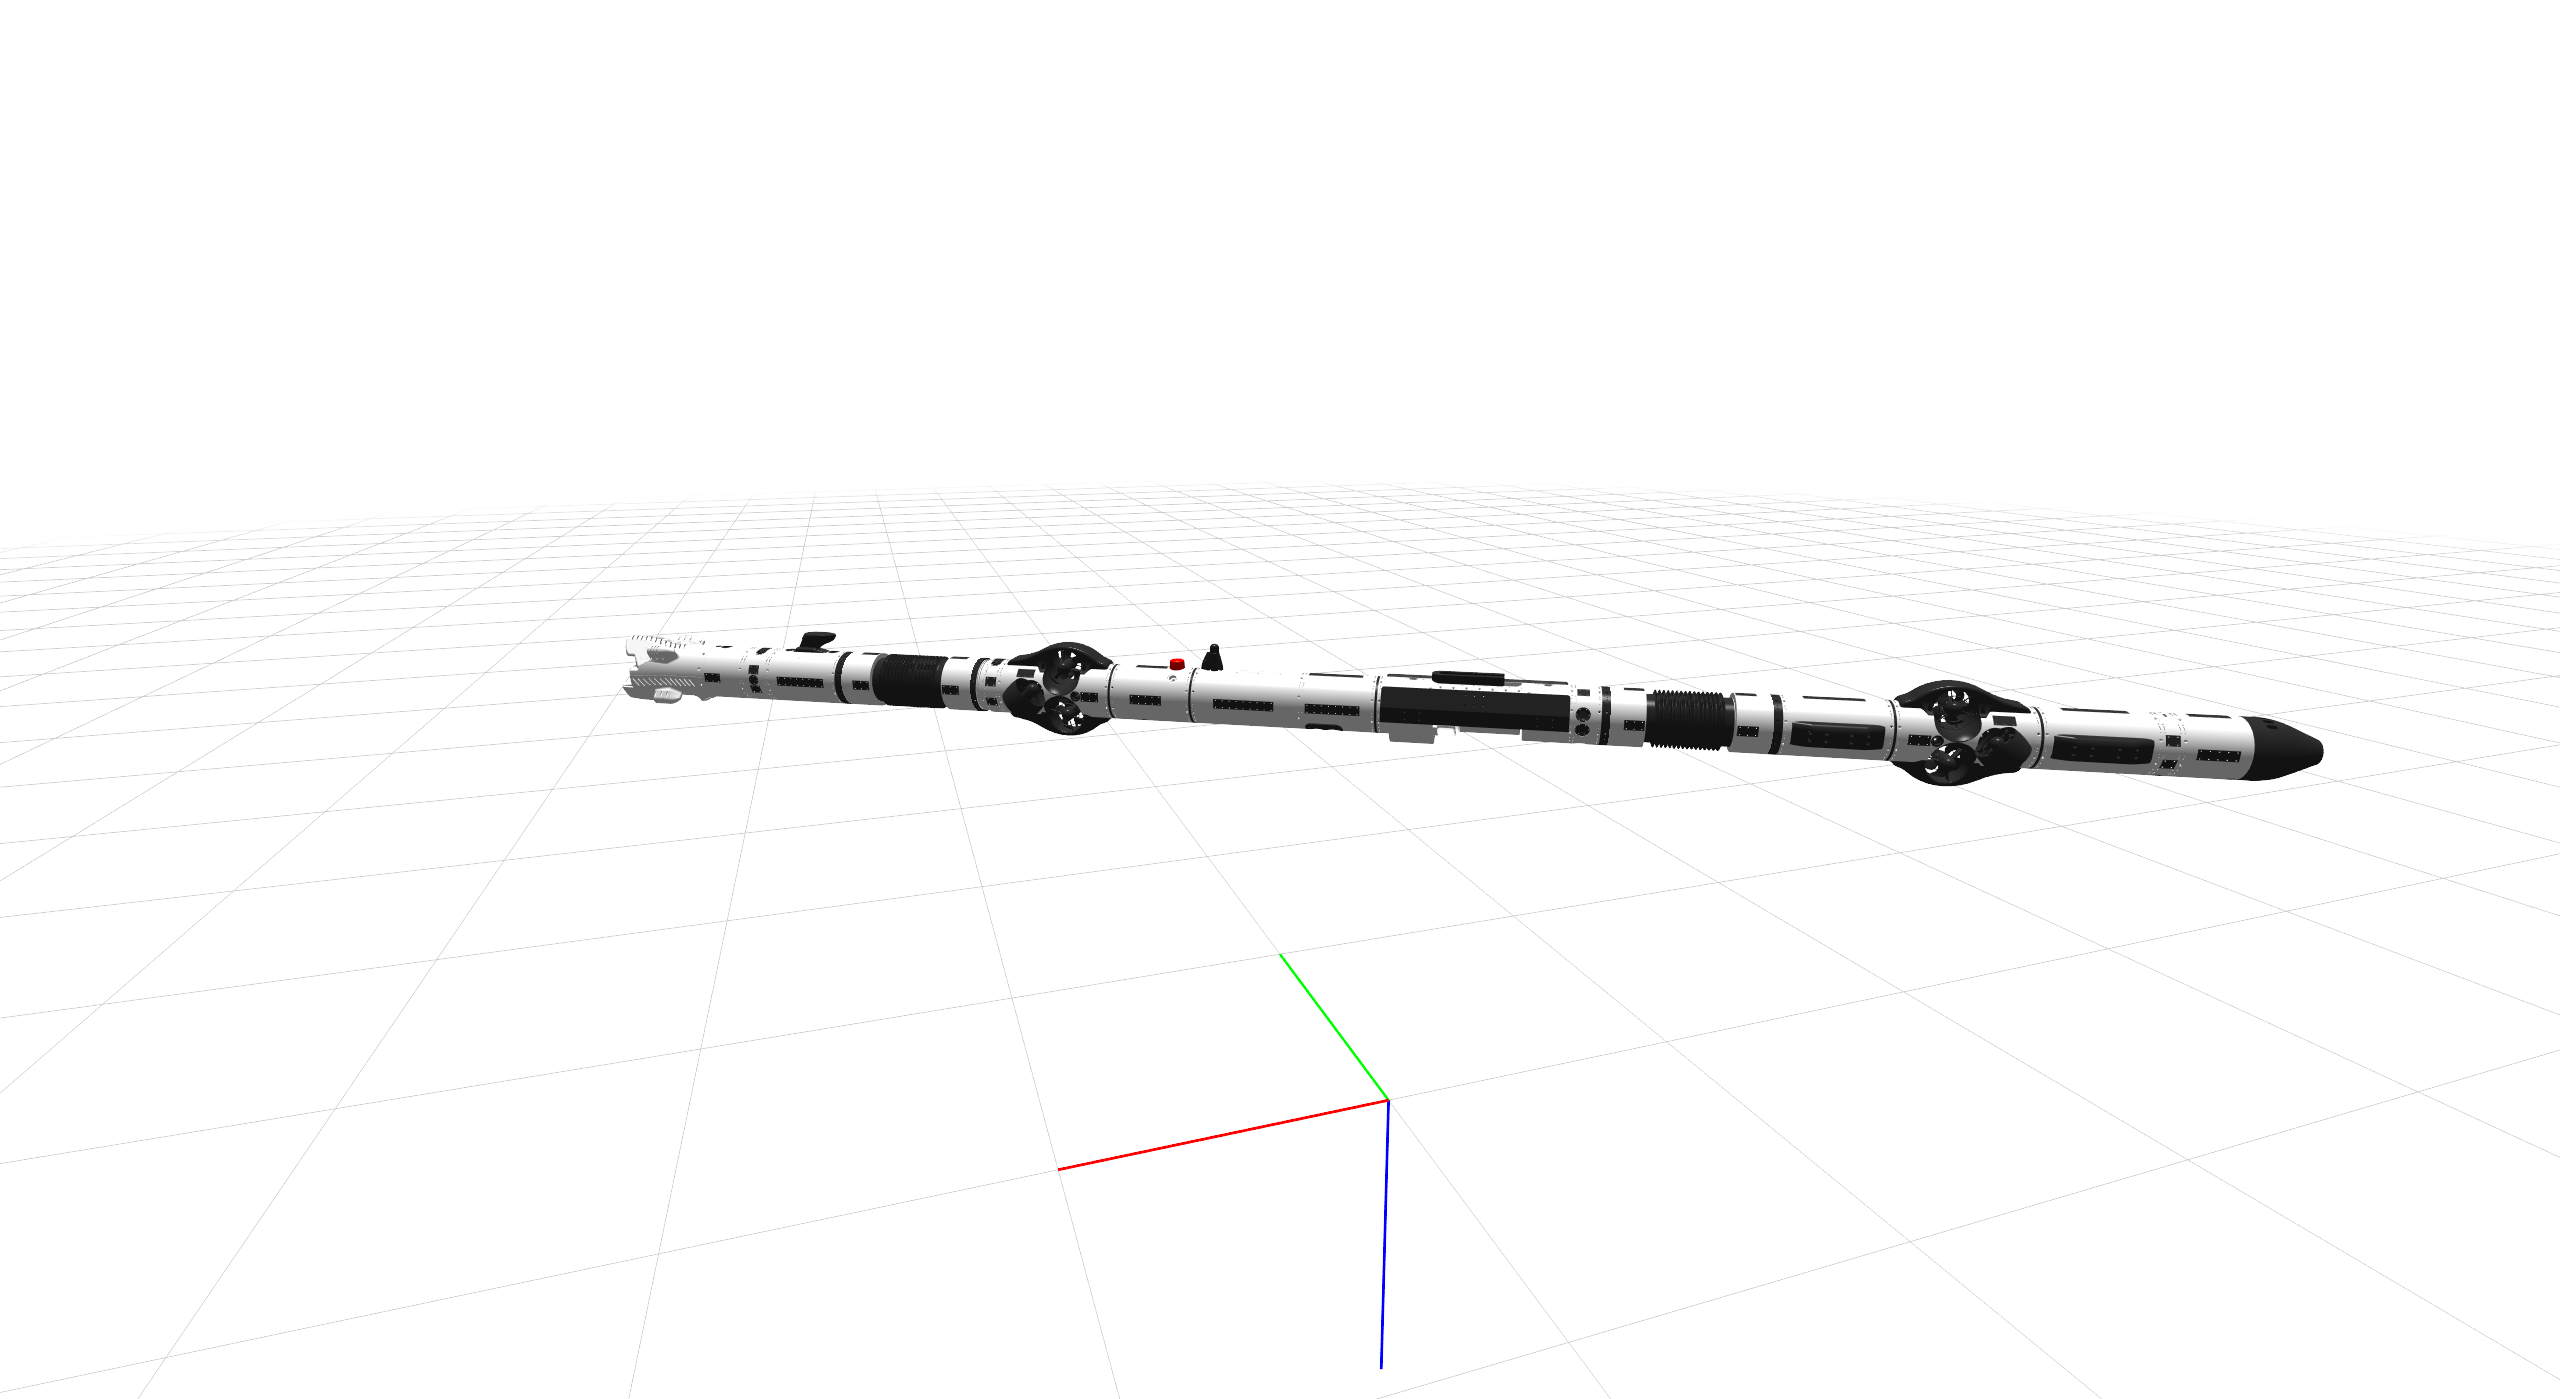
\includegraphics[width=\textwidth]{assets/eely-visualizer.png}
    \caption{A screenshot of the Eelume visualizer.}
    \label{fig:eelume:visualizer}
\end{figure}

\FloatBarrier

\section{EelyControlKit}

\gls{eck} refers to a C++ library developed as part of this thesis for 
controlling the Eelume robot.  
To better understand the purpose and functionality of this library, some 
background information on the internal workings of the Eelume robot is 
necessary.

The Eelume robot is controlled using a low-level \gls{api} provided by Eelume AS in 
early 2025. This \gls{api} grants access to the internal \gls{can} bus, which 
is used for communication with the robot's thrusters, joints, and sensors. 
While the \gls{api} allows for sending arbitrary messages over this bus, it 
also includes a set of functions for transmitting predefined messages used by 
various robot components. For example, setting thrust and joint torque 
references requires sending multiple messages across the bus for the thrusters 
to correctly adjust their internal references.

The \gls{api} is implemented in C/C++ and communicates with the robot via an 
Ethernet connection. Due to its low-level nature, significant additional code 
was required to implement the \gls{tpc} framework, including modules for lower-
level controllers, mathematical operations, task definitions, and kinematic 
and dynamic modeling. This codebase, built atop the low-level \gls{api}, is 
referred to as \gls{eck}.

A key design decision was to develop this control kit as a reusable library. 
The goal is to facilitate the development of a wide range of controllers, not 
only task-priority controllers, by providing the necessary tools and 
mathematical infrastructure. The library is written in C++, partly to align 
with the low-level API and partly due to the computational demands of task-
priority control. Using C++ ensures fast runtimes, albeit at the cost of 
longer compile times. Since \gls{eck} is built as a library, it can be 
compiled once and linked for subsequent use, enabling faster compilation and 
maintaining clean abstractions.

% -----------------------------------------------------------------------------
\subsection{Features}

% connection to the Eelume robot
One of the primary features of \gls{eck} is a connection class that 
encapsulates the communication between the Eelume robot and external software. 
This class handles all necessary setup, message subscriptions, data parsing, 
and formatting for transmission. It exposes a \textit{connect} function that 
returns an object representing the connection if successful. Throughout the 
codebase, C++17 \textit{optionals} are used to elegantly manage unexpected 
errors and invalid states. Additionally, the connection class provides 
functions for setting references for thrusters and joint motors, enabling 
quick testing without rewriting code.

% kinematics and jacobians and (B) matrix
Another major contribution is the kinematics class. This class represents the 
robot’s kinematic model and provides access to a range of methods rooted in 
kinematics. It computes and returns transformations between frames and calculates 
Jacobians. It is extensively used in computing task Jacobians for task-
priority control. Combined with a specification of the thruster configuration, 
the kinematics class enables computation of the thruster allocation matrix \(\
bm{B}\) in \autoref{eq:modeling:Bdef}, which is then used for simple pseudo-
inverse-based thruster allocation.

% a set of controllers
Among the features of \gls{eck} is a collection of pre-defined controllers. 
This includes a simple \gls{pd} controller, a \gls{pd+} controller, and 
velocity-level task-priority controllers. All controllers adhere to a common 
interface, which allows switching between controllers at runtime instead of 
compile time, if desired. The implemented task-priority controller is general 
and supports arbitrary null-space projection methods, with standard successive 
and augmented methods included. A \textit{task} class is also provided, which 
automatically computes task Jacobians for position and orientation tasks using 
the given kinematic model.

% mathematical and utility functions
A suite of mathematical and utility functions is also included. These range 
from basic operations, such as rotation matrices and skew-symmetric products, 
to more advanced tools like a Runge-Kutta integrator that accepts arbitrary 
lambda functions. A reference generator is also implemented using this 
integrator, which allows for low-pass filtering of references and outputs 
desired task values along with their derivatives for use in control algorithms.

% -----------------------------------------------------------------------------
\section{Simulator}

As part of \gls{eck}, a built-in simulator was implemented. The simulator is 
constructed using the same interface as the Eelume connection class, enabling 
seamless switching between running on the simulator and the actual robot 
without recompiling the code. Although simulators for the Eelume robot already 
exist, none were found to align fully with the kinematic models and 
conventions adopted in this thesis. Certain assumptions must always be made 
when designing a simulator, such as the numbering of joints and thrusters or 
the mathematical form of the dynamic equations. To ensure compatibility with 
the assumptions and conventions used throughout this work, it was ultimately 
more efficient to implement the simulator from scratch. Given that much of the 
functionality for computing Jacobians and kinematics was already in place, 
adding the dynamics required relatively little additional effort.

A dynamic model of the Eelume robot was developed specifically for use in this 
simulator. The model aims to provide a reasonable approximation of the robot’s 
dynamics, while avoiding time-intensive steps in the identification process, 
such as capturing fluid memory effects or hydrodynamic coupling. The model is 
based on the assumption that each link can be approximated as a cylinder with 
a radius of \(10\) cm. The added mass and linear damping are modeled as 
described in \autoref{sec:hydrodynamics}, and the kinematics follow the 
parameters presented in \autoref{tab:eelume:keynumbers}.

The simulator supports arbitrary time steps and allows the controller and 
simulator to run at different frequencies. This capability provides a more 
realistic simulation of the interplay between the controller and the physical 
system. The integration is performed using a fourth-order Runge-Kutta method 
with a time step as small as 1 ms, enabling faster-than-real-time execution 
for rapid testing. The simulator can be connected to the Eelume Visualizer, 
enabling real-time feedback that facilitates the identification of bugs and 
implementation issues during development.

The simulator proved invaluable in the development of task-priority controllers.
Thanks to the implemented abstractions, it enabled development and testing 
without requiring a physical connection to the Eelume robot. This 
significantly reduced the amount of test time and manpower needed. While the 
model is not perfectly accurate, it provides a sufficiently realistic 
approximation to understand controller behavior prior to real-world testing. 
This helps avoid cases where a controller may act too aggressively or operate 
near kinematic limits.

\section{Conclusion}

The development of the Eelume Visualizer, \gls{eck}, and the 
built-in simulator represent significant contributions of this thesis. Together,
they form a comprehensive software ecosystem that supports visualization, 
control, and simulation of the Eelume robot. The Visualizer provides intuitive 
and real-time insight into the robot's configuration and behavior, aiding both 
experimentation and presentation. Its integration with external tools and 
rendering capabilities has proven valuable for development and debugging. 

\gls{eck} offers a structured and extensible control framework built in C++, 
enabling the implementation and testing of advanced control strategies such as 
task-priority control. It abstracts low-level communication with the robot and 
provides modular components for kinematics, dynamics, and control. The 
accompanying simulator, tightly integrated with \gls{eck}, allows for high-
fidelity testing without physical hardware. By faithfully modeling the robot's 
dynamics and maintaining compatibility with the same interface used for real-
world operation, the simulator has been instrumental in efficient controller 
development, significantly reducing testing time and risk.

